\documentclass[UTF8]{ctexart}
\usepackage{arxiv}
\usepackage{amsmath}
\usepackage{amssymb}
\usepackage{array}
\usepackage{booktabs}
\usepackage{float}
\usepackage{graphicx}
\usepackage{hyperref}
\usepackage{subcaption}
\usepackage{tabularx}
\usepackage{titlesec}
\usepackage{url}

\renewcommand{\headeright}{李承锦}
\renewcommand{\undertitle}{\mbox{}}
\renewcommand{\shorttitle}{机器学习课程算法仿真报告}
\renewcommand{\refname}{参考文献}
\renewcommand{\abstractname}{摘要}

\hypersetup{
  colorlinks=true,
  linkcolor=black,
  citecolor=black,
  urlcolor=blue
}

\makeatletter
\def\keywordname{{\bfseries 关键词}}
\makeatother

\titleformat{\section}{\large\bfseries\raggedright}{\thesection}{0.75em}{}
\titleformat{\subsection}{\normalsize\bfseries\raggedright}{\thesubsection}{0.75em}{}
\titlespacing*{\section}{0pt}{1.2\baselineskip}{0.4\baselineskip}
\titlespacing*{\subsection}{0pt}{0.9\baselineskip}{0.3\baselineskip}

\title{机器学习课程算法仿真与对比分析报告\\基于 K-means、SVM、BP 网络与 RBF 网络}
\author{
李承锦（学号：202521011635） \\
\texttt{https://github.com/ChengjinLii/machine\_learning\_project}
}
\date{2026 年 4 月 20 日}

\begin{document}
\maketitle

\begin{abstract}
本文围绕机器学习课程中的典型算法，选取 K-means、支持向量机（SVM）、BP 神经网络和径向基函数（RBF）网络四类方法进行仿真，并补充参数敏感性与结构对比实验。实验数据来自 Iris、Wine 和 Fashion-MNIST 三个开源数据集，数据获取、预处理、训练、评估与可视化均在同一仓库中完成，代码开源地址为 \url{https://github.com/ChengjinLii/machine_learning_project}。

实验结果表明：在 Iris 数据集上，采用 $K=3$ 的 K-means 聚类可得到 0.6201 的调整兰德指数和 0.6595 的归一化互信息；在 Wine 数据集上，RBF 核 SVM 的测试准确率为 97.78\%，基于 K-means 选中心的 RBF 网络在 9 个隐层中心时测试准确率为 100\%；在 Fashion-MNIST 子集上，三层隐藏结构的 BP/MLP 网络测试准确率为 86.275\%。附加实验表明，聚类内部指标与外部一致性指标之间存在差异，RBF 网络对隐层中心数敏感，BP 网络则呈现出精度与计算代价之间的折中关系。
\end{abstract}

\keywords{机器学习, K-means, 支持向量机, BP 神经网络, RBF 网络}

\section{引言}
机器学习课程通常围绕监督学习、无监督学习和神经网络三条主线展开。为将课件中的理论内容落实为可复现的实验结果，本文从课程资料中选取四类代表性算法完成仿真：无监督聚类中的 K-means，统计学习中的支持向量机，前馈神经网络中的 BP 网络，以及具备局部基函数建模能力的 RBF 网络。

除给出主实验结果外，本文还补充了多组对比实验，以分析模型在不同参数设置下的性能变化。具体而言，K-means 部分比较不同簇数 $K$ 的聚类结果，SVM 部分比较不同核函数，RBF 网络部分比较不同隐层中心数，BP 网络部分比较不同多层感知机结构。通过这些实验，可进一步考察各类算法在不同数据集和参数条件下的表现。

\section{算法原理与实验对象}

\subsection{K-means 聚类}
K-means 是最经典的原型聚类算法之一，其核心思想是给定簇数 $K$ 后，交替执行“样本分配”和“中心更新”两个步骤，以最小化簇内平方误差和 \cite{macqueen1967}：
\begin{equation}
\min_{\{\mathcal{C}_k\}, \{\mu_k\}}
\sum_{k=1}^{K} \sum_{x_i \in \mathcal{C}_k} \|x_i - \mu_k\|_2^2 .
\end{equation}
K-means 不依赖标签信息，适用于分析样本的自然分组结构。本文在 Iris 数据集上验证其聚类效果，并比较不同 $K$ 值对应的性能变化。

\subsection{支持向量机}
支持向量机通过最大化分类间隔寻找最优分离超平面，是统计学习理论中极具代表性的二分类方法 \cite{cortes1995svm}。对于线性可分情形，其基本优化问题为
\begin{equation}
\min_{w,b} \frac{1}{2}\|w\|_2^2,
\qquad
\text{s.t.}\quad y_i(w^\top x_i + b)\ge 1.
\end{equation}
实际问题往往并非线性可分，因此可通过核技巧构造隐式高维映射。本文在 Wine 数据集上比较线性核、多项式核、Sigmoid 核和 RBF 核的表现。

\subsection{BP 神经网络}
BP 神经网络通过误差反向传播求解多层前馈网络参数 \cite{rumelhart1986bp}。在输出层得到损失后，梯度逐层向前传播，并据此更新网络权值。本文采用多层感知机（MLP）作为 BP 网络的工程实现，该结构与课件中的“输入层-隐层-输出层”模型一致，便于在图像分类任务上进行对比实验。

\subsection{RBF 网络}
RBF 网络通常由输入层、RBF 隐层和线性输出层构成。若隐层采用高斯基函数，则第 $j$ 个单元的响应可写为 \cite{moody1989rbf}
\begin{equation}
\phi_j(x)=\exp\left(-\gamma \|x-c_j\|_2^2\right),
\end{equation}
其中 $c_j$ 为第 $j$ 个中心。课程课件中明确介绍了“先以 K-means 确定中心，再通过最小二乘法确定输出层权值”的训练思路，本文严格按照这一思路实现多分类 RBF 网络，并比较不同隐层中心数下的表现。

\subsection{数据集说明}
本文使用 3 个公开数据集，覆盖传统表格数据与图像数据两类任务场景。

\begin{table}[H]
\centering
\caption{本文使用的数据集概况}
\label{tab:dataset-summary}
\small
\begin{tabular}{lcccccc}
\toprule
数据集 & 总样本数 & 特征维度 & 类别数 & 训练样本 & 测试样本 & 来源 \\
\midrule
Iris & 150 & 4 & 3 & -- & -- & UCI \\
Wine & 178 & 13 & 3 & 133 & 45 & UCI \\
Fashion-MNIST & 70000 & 784 & 10 & 12000 & 4000 & Zalando 发布数据 \\
\bottomrule
\end{tabular}
\end{table}

Iris 数据集最早由 Fisher 用于多变量分类研究 \cite{fisher1936iris}，并可从 UCI 机器学习仓库获取 \cite{uciiris}。Wine 数据集同样来自 UCI 机器学习仓库 \cite{uciwine}，包含三类葡萄酒在 13 个理化属性上的测量结果。Fashion-MNIST 数据集由 Xiao 等提出 \cite{xiao2017fashion}，常用作入门级图像分类基准。

\section{实验环境与评价指标}

\subsection{软件环境}
实验在统一的 Python/conda 环境中完成。为支持数据读取、数值计算、模型训练与结果可视化，环境中需包含 \texttt{numpy}、\texttt{pandas}、\texttt{matplotlib}、\texttt{scikit-learn}、\texttt{scipy}、\texttt{seaborn} 和 \texttt{requests} 等依赖库。为保证各算法实验在同一配置下运行，本文采用统一环境安装和管理上述依赖，以减少库版本差异对实验结果的影响。

\subsection{预处理与评价指标}
不同实验采用统一的预处理方案。Iris 与 Wine 数据均进行标准化处理，以避免量纲差异影响距离或间隔计算；Fashion-MNIST 图像像素被线性归一化到 $[0,1]$ 区间。监督学习实验采用准确率（Accuracy）和宏平均 $F_1$ 值（Macro-F1）评估：
\begin{equation}
\text{Accuracy}=\frac{1}{N}\sum_{i=1}^{N}\mathbf{1}(\hat{y}_i=y_i).
\end{equation}
对于多分类任务，宏平均 $F_1$ 先分别计算各类别的 $F_1$ 值，再取算术平均。

聚类实验额外采用 3 个指标：
\begin{itemize}
\item 轮廓系数（Silhouette），反映簇内紧凑性与簇间分离性。
\item 调整兰德指数（ARI），评估聚类结果与真实类别的一致性。
\item 归一化互信息（NMI），评估聚类标签与真实标签的信息共享程度。
\end{itemize}

\section{主实验结果}

\subsection{总体结果汇总}
四类算法在各自任务上的核心结果如表 \ref{tab:main-summary} 所示。表格数据上的监督分类性能整体较高，其中 RBF 网络在该训练/测试划分下取得了 100\% 的测试准确率；对于类别更多、样本形态更复杂的 Fashion-MNIST，BP 网络的准确率低于 Wine 分类任务，但仍保持在较高水平。

\begin{table}[H]
\centering
\caption{四类算法主实验结果汇总}
\label{tab:main-summary}
\small
\begin{tabular}{lccccc}
\toprule
算法 & 数据集 & 关键设置 & Accuracy / ARI & Macro-F1 / NMI & 备注 \\
\midrule
K-means & Iris & $K=3$ & ARI = 0.6201 & NMI = 0.6595 & Silhouette = 0.4590 \\
SVM & Wine & RBF 核 & 0.9778 & 0.9765 & 最优核函数 \\
RBF 网络 & Wine & 9 个中心 & 1.0000 & 1.0000 & 该划分下最高 \\
BP 网络 & Fashion-MNIST & MLP(256,128,64) & 0.8628 & 0.8631 & 30 个 epoch \\
\bottomrule
\end{tabular}
\end{table}

\subsection{K-means 聚类结果}
图 \ref{fig:kmeans-clusters} 展示了 Iris 数据集在 PCA 二维投影下的真实标签与聚类结果。setosa 类基本单独成簇，而 versicolor 与 virginica 存在一定重叠，因此 K-means 难以完全恢复真实类别边界。该实验的 ARI 为 0.6201，说明聚类结果与真实类别之间具有较强一致性。

\begin{figure}[H]
\centering
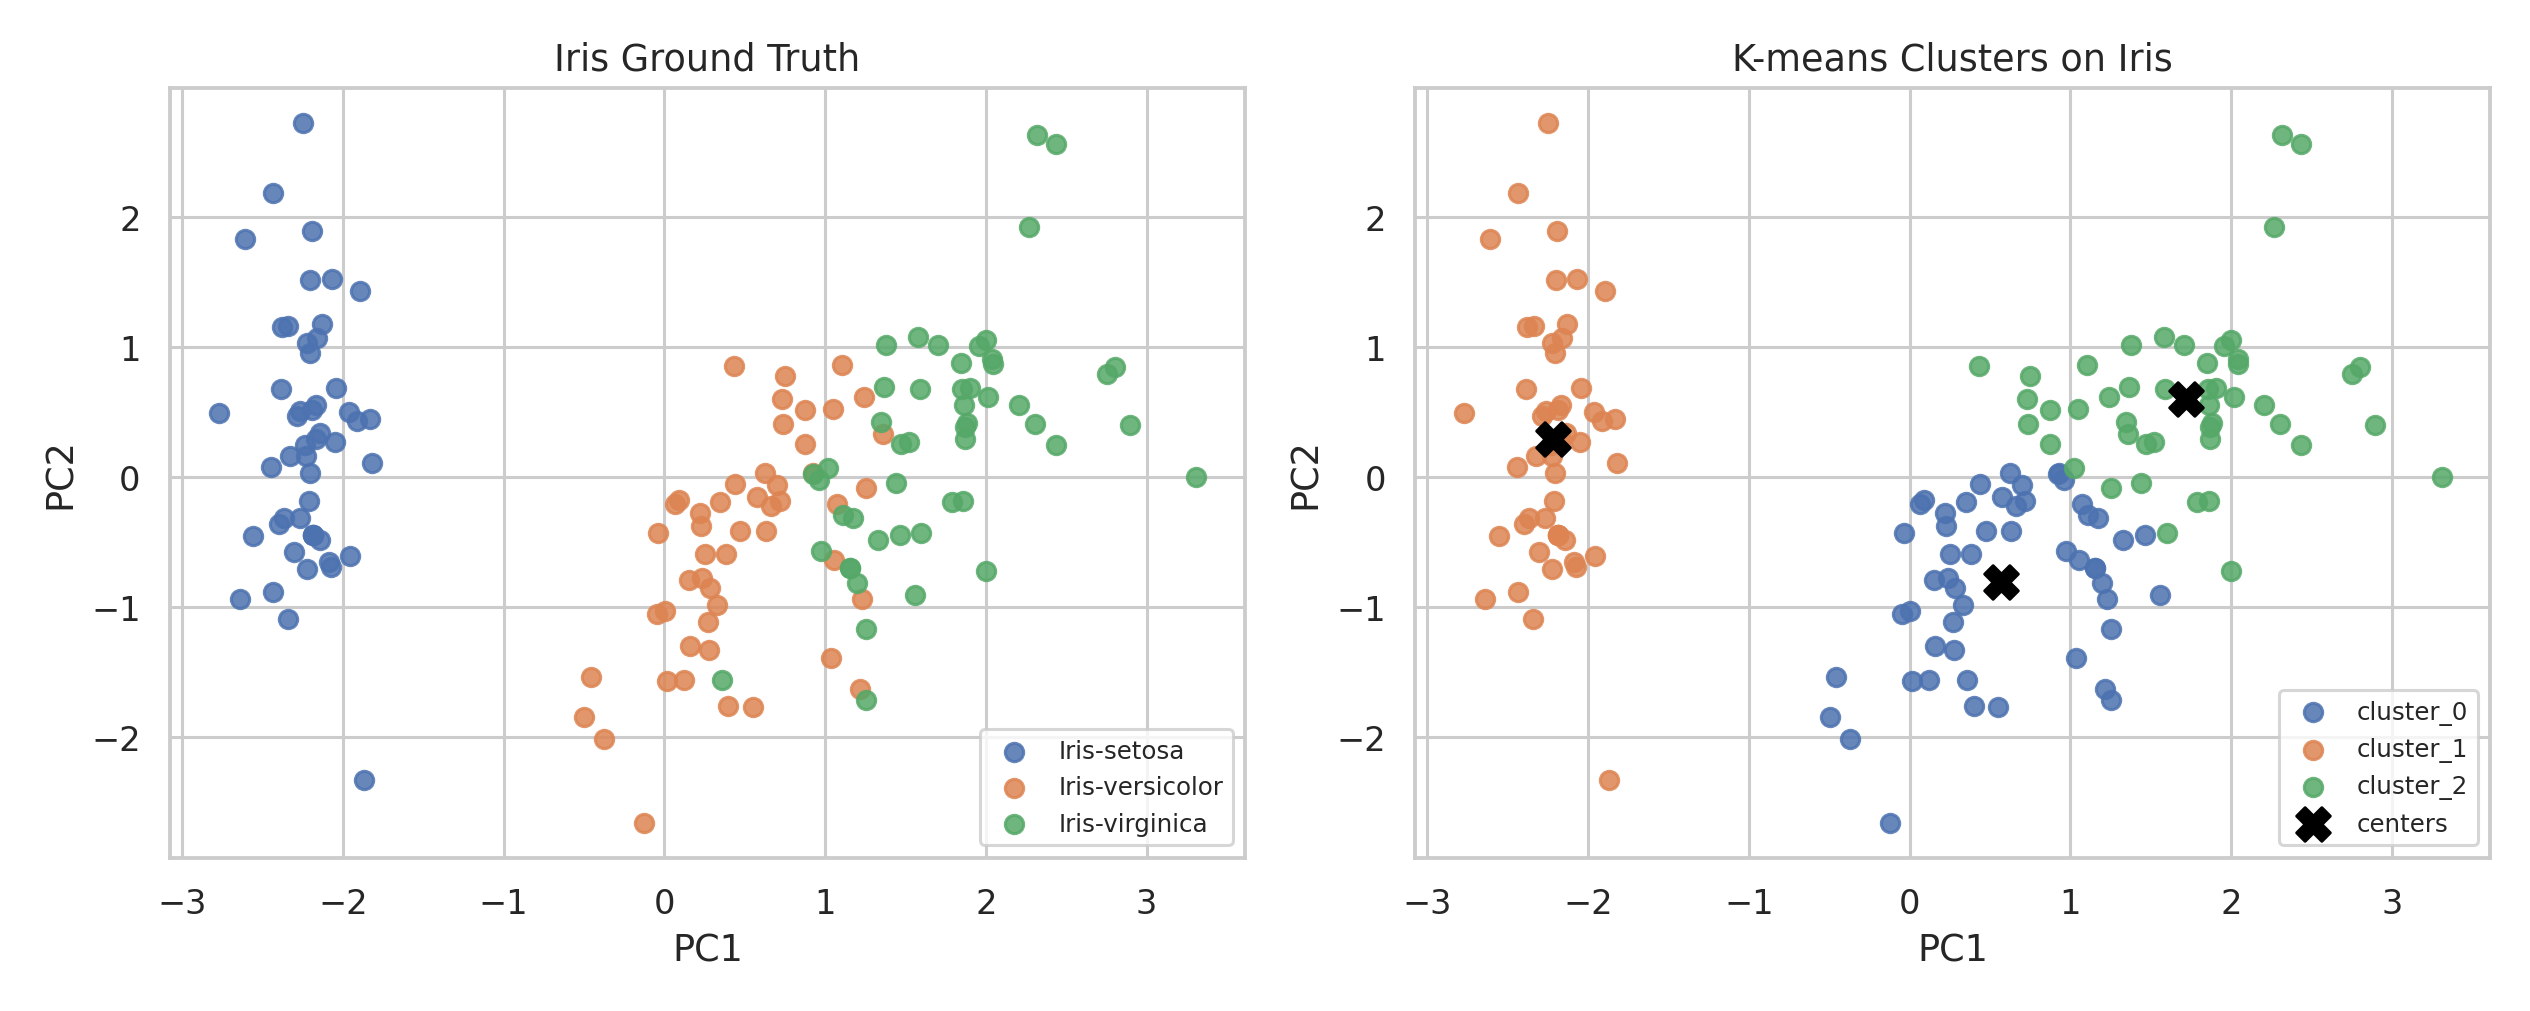
\includegraphics[width=0.92\linewidth]{../results/figures/kmeans_iris_clusters.png}
\caption{Iris 数据集上的 K-means 聚类结果}
\label{fig:kmeans-clusters}
\end{figure}

\subsection{SVM 分类结果}
SVM 主实验采用 RBF 核，其在 Wine 测试集上的准确率为 97.78\%，宏平均 $F_1$ 值为 0.9765。图 \ref{fig:svm-cm} 的混淆矩阵显示，大多数样本均被正确分类，仅存在少量跨类别误判。对于样本量较小且类别结构较清晰的表格数据，SVM 具有稳定的分类性能。

\begin{figure}[H]
\centering
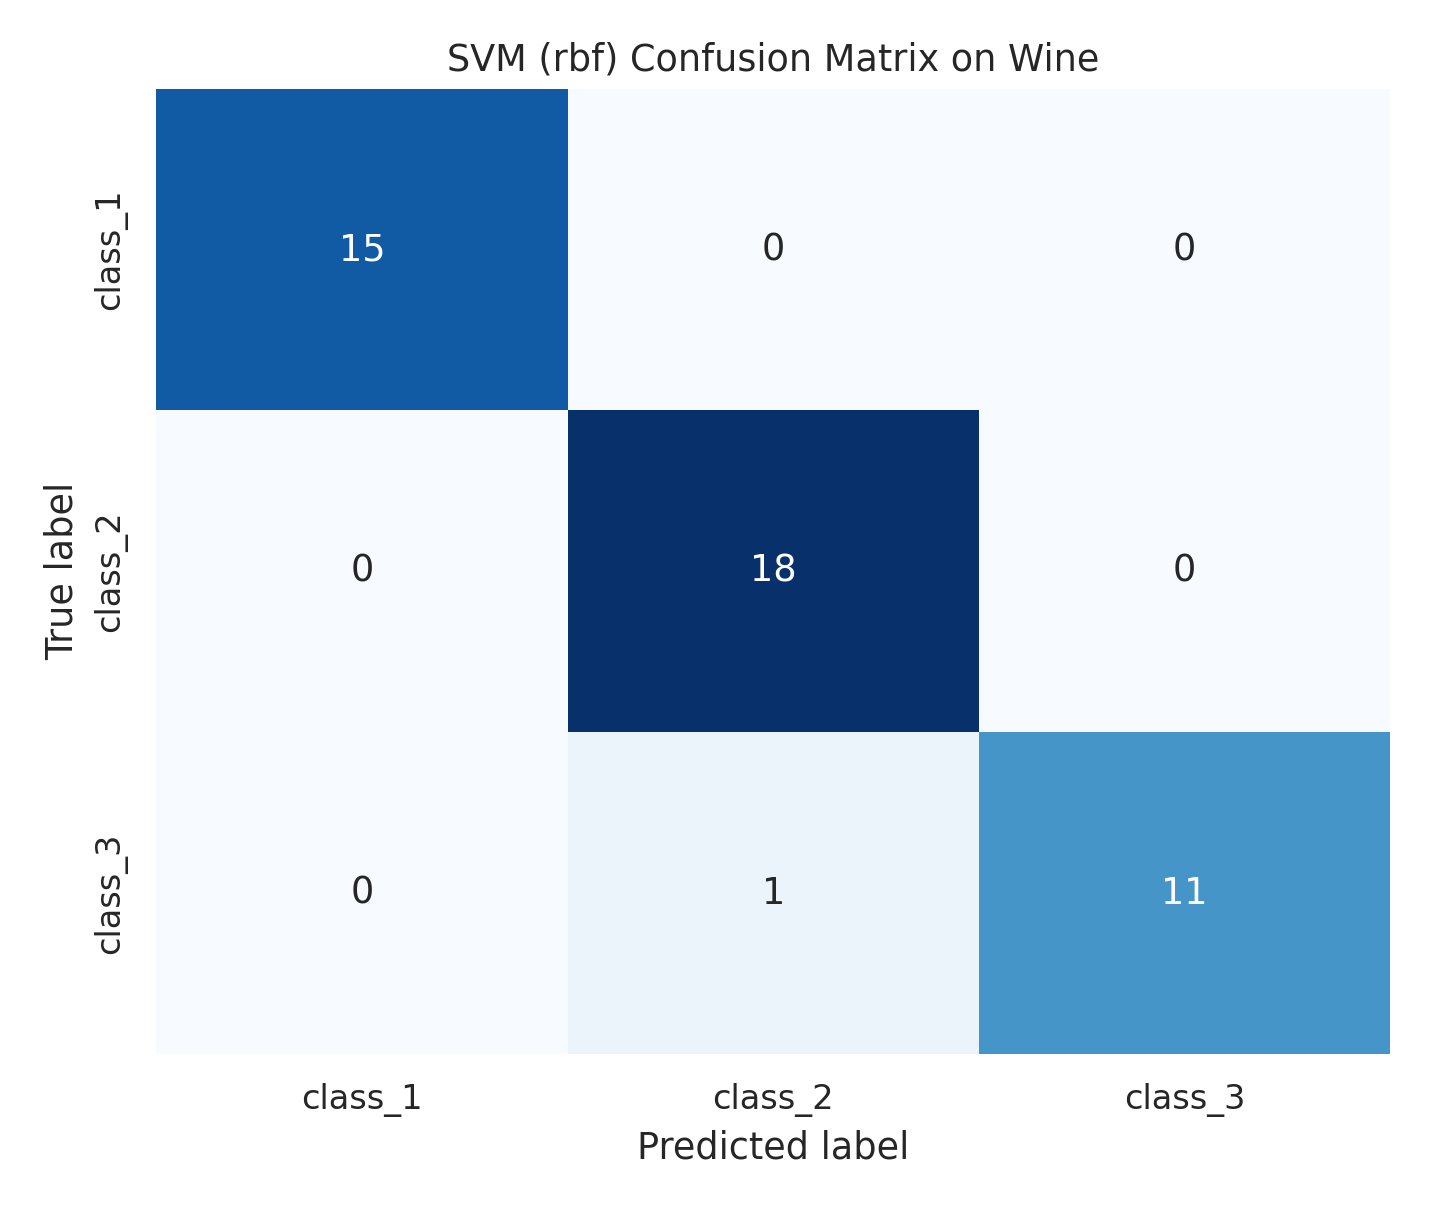
\includegraphics[width=0.70\linewidth]{../results/figures/svm_wine_confusion.png}
\caption{Wine 数据集上的 SVM 混淆矩阵}
\label{fig:svm-cm}
\end{figure}

\subsection{RBF 网络结果}
图 \ref{fig:rbf-cm} 给出了 RBF 网络在 Wine 数据集上的混淆矩阵。该实现与课件中“先聚类取中心，再线性输出”的结构一致。当隐层中心数取 9 时，测试集准确率和宏平均 $F_1$ 值均达到 1.0000，表明局部基函数映射能够在该数据集上形成有效的判别边界。

\begin{figure}[H]
\centering
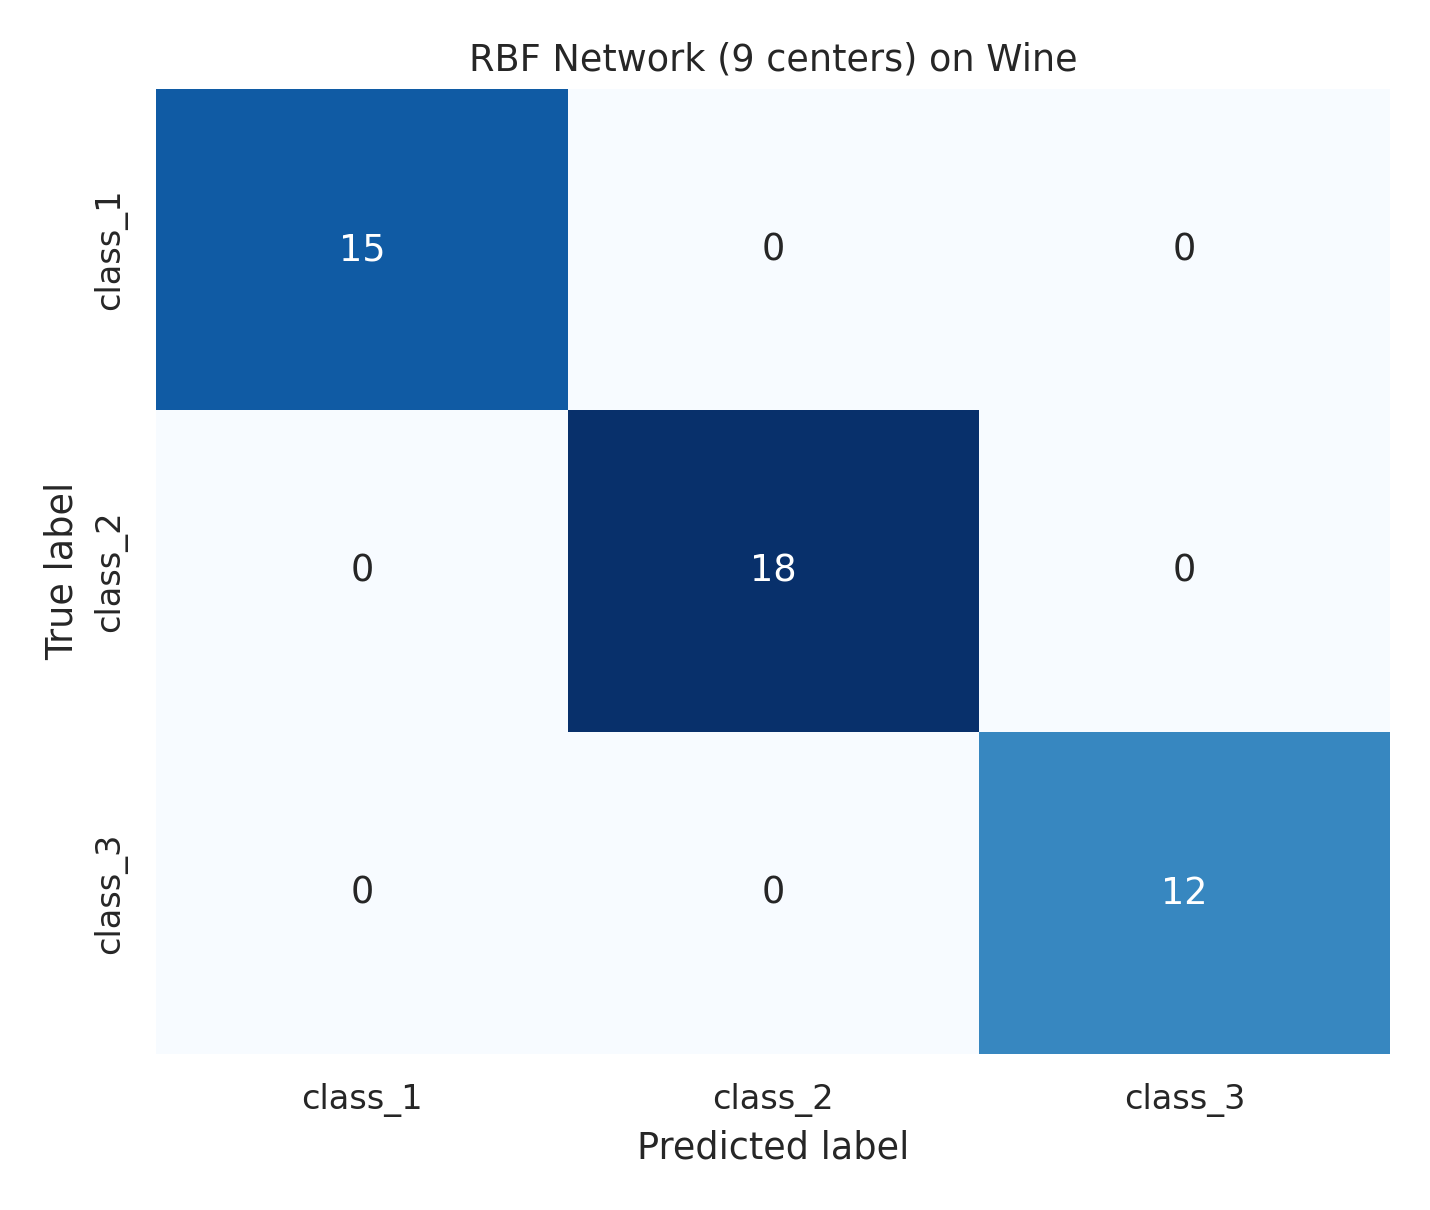
\includegraphics[width=0.70\linewidth]{../results/figures/rbf_wine_confusion.png}
\caption{Wine 数据集上的 RBF 网络混淆矩阵}
\label{fig:rbf-cm}
\end{figure}

\subsection{BP 网络结果}
BP 网络采用 Fashion-MNIST 子集进行训练与测试，测试性能最高的结构为 \texttt{MLP(256,128,64)}。如图 \ref{fig:mlp-loss} 所示，训练损失随 epoch 增加而持续下降，表明网络在该样本规模上能够收敛。图 \ref{fig:mlp-cm} 的混淆矩阵显示，服饰图像中的相近类别仍存在较多混淆，例如 T-shirt/top、Shirt 与 Pullover 之间的误分较为集中，这与图像本身的细粒度相似性一致。

\begin{figure}[H]
\centering
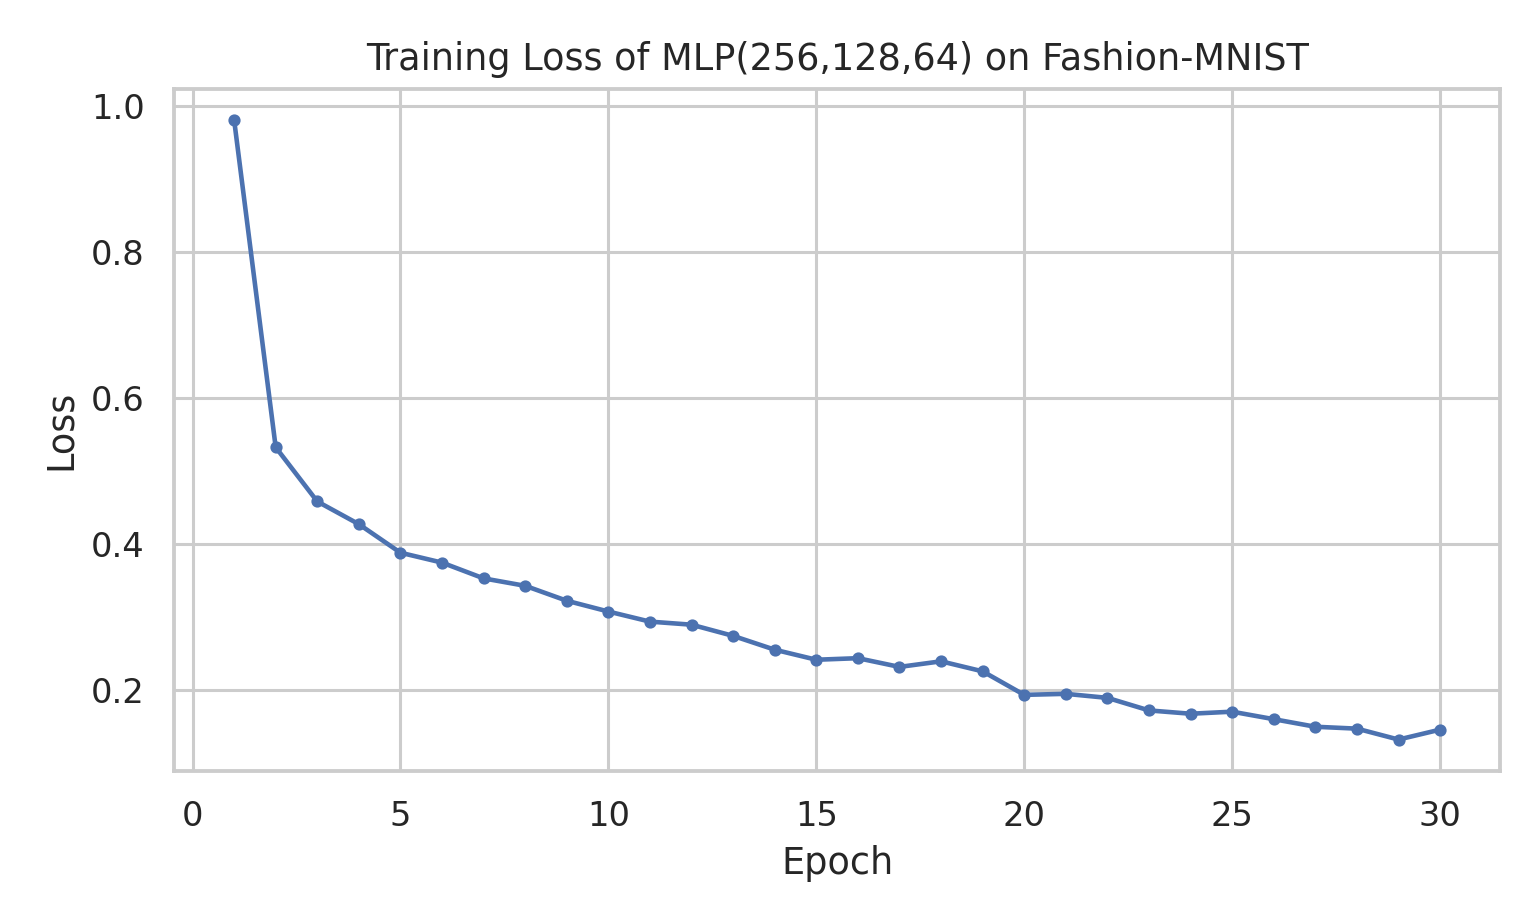
\includegraphics[width=0.72\linewidth]{../results/figures/mlp_fashion_loss.png}
\caption{Fashion-MNIST 子集上的 BP/MLP 训练损失曲线}
\label{fig:mlp-loss}
\end{figure}

\begin{figure}[H]
\centering
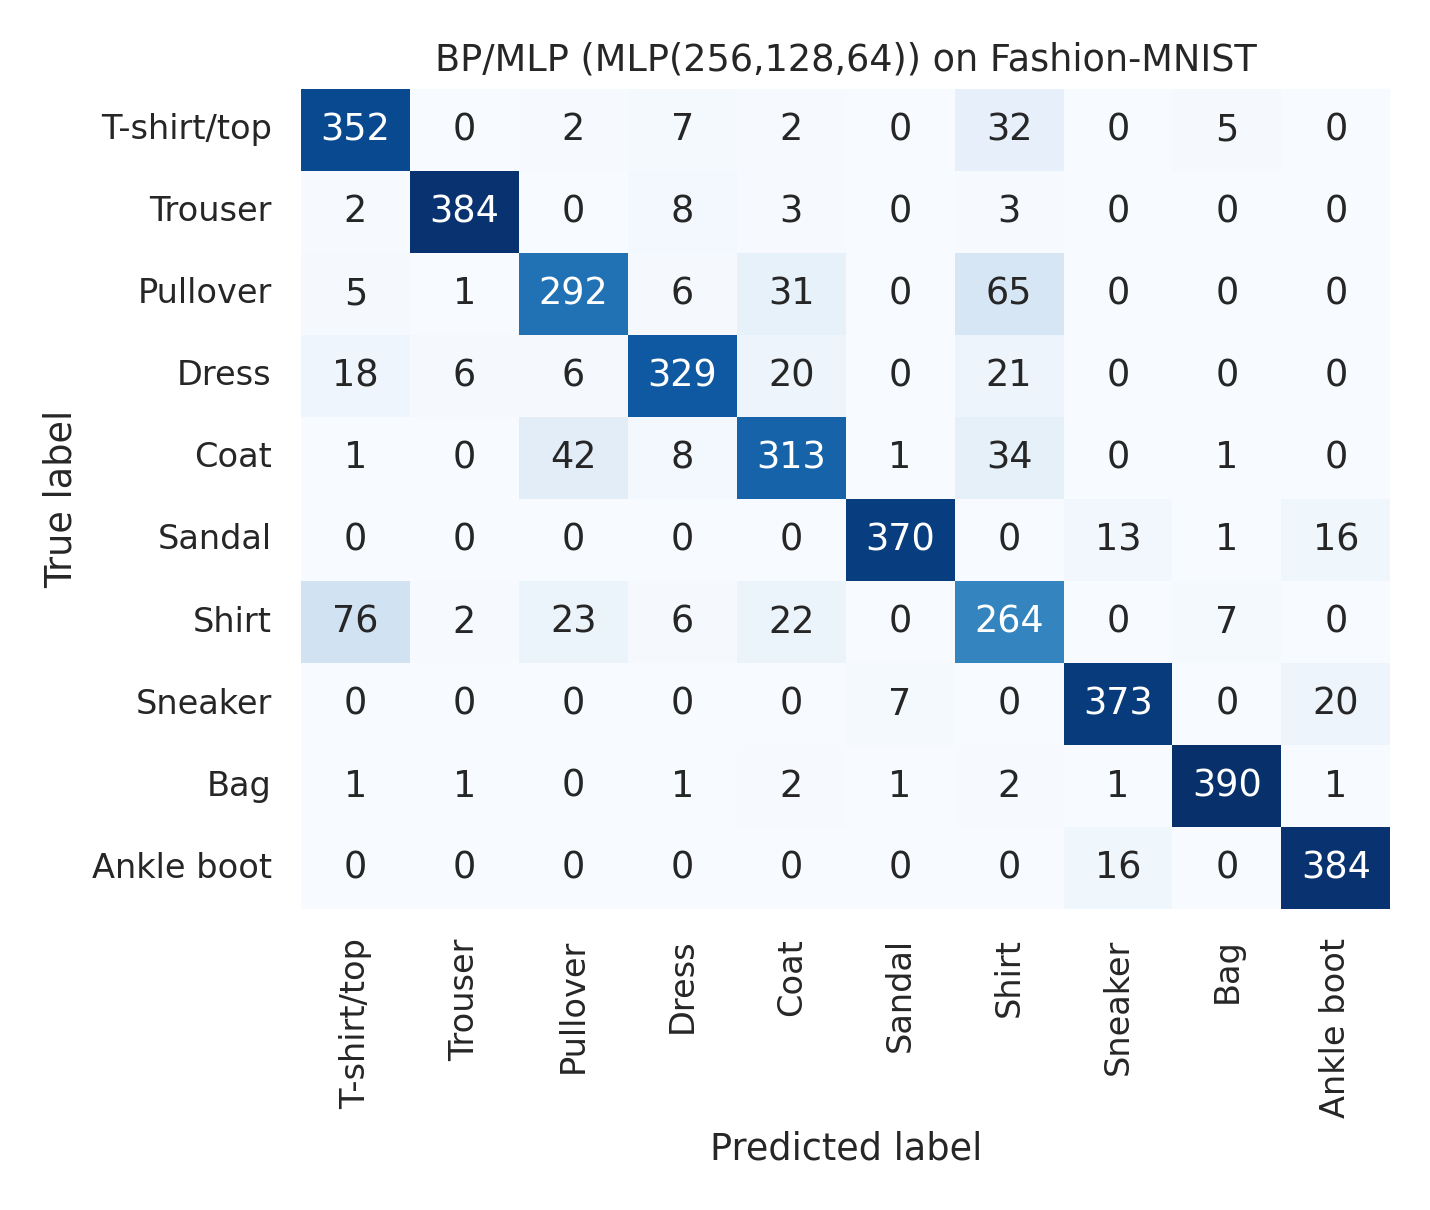
\includegraphics[width=0.90\linewidth]{../results/figures/mlp_fashion_confusion.png}
\caption{Fashion-MNIST 子集上的 BP/MLP 混淆矩阵}
\label{fig:mlp-cm}
\end{figure}

\section{附加对比实验与分析}

\subsection{K-means 的簇数敏感性}
为分析簇数选择对聚类结果的影响，本文进一步比较了 $K=2,3,4,5,6$ 五种设置。对应结果见表 \ref{tab:kmeans-sweep} 和图 \ref{fig:kmeans-sweep}。

\begin{table}[H]
\centering
\caption{Iris 数据集上 K-means 的不同簇数比较}
\label{tab:kmeans-sweep}
\small
\begin{tabular}{ccccc}
\toprule
$K$ & Inertia & Silhouette & ARI & NMI \\
\midrule
2 & 223.7320 & 0.5802 & 0.5681 & 0.7337 \\
3 & 140.9658 & 0.4590 & 0.6201 & 0.6595 \\
4 & 114.3885 & 0.3874 & 0.4706 & 0.5967 \\
5 & 91.0756 & 0.3516 & 0.4167 & 0.5873 \\
6 & 80.1667 & 0.3259 & 0.3512 & 0.5374 \\
\bottomrule
\end{tabular}
\end{table}

\begin{figure}[H]
\centering
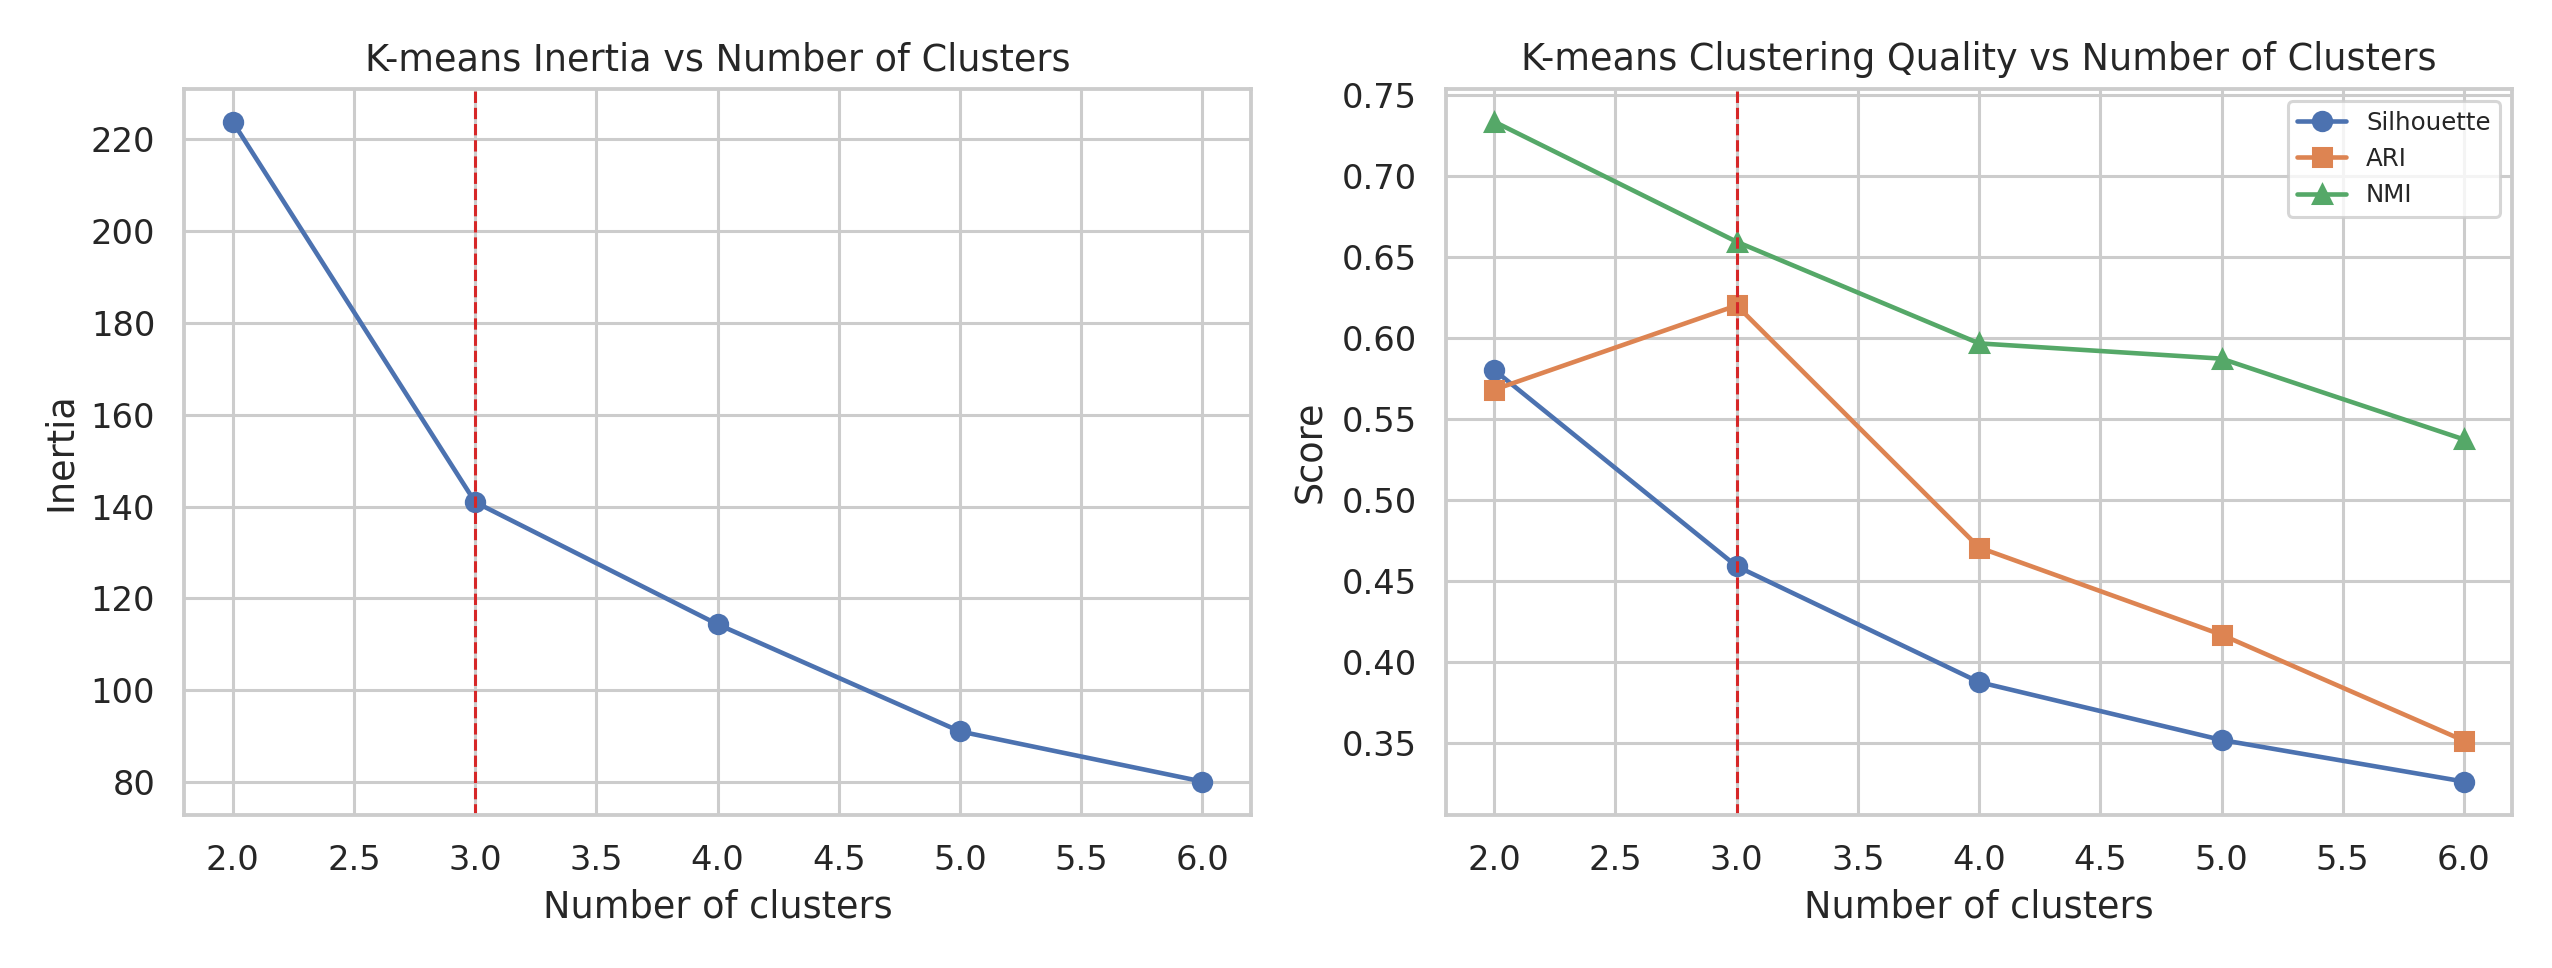
\includegraphics[width=0.92\linewidth]{../results/figures/kmeans_iris_k_sweep.png}
\caption{Iris 数据集上 K-means 的簇数扫描结果}
\label{fig:kmeans-sweep}
\end{figure}

若仅考察轮廓系数，则 $K=2$ 优于 $K=3$；若引入真实标签进行外部评估，则 $K=3$ 的 ARI 最高。该结果表明，内部聚类指标更偏向于刻画簇内紧凑性，而外部一致性指标更关注聚类结果与真实类别划分之间的对应关系。因此，聚类任务的评价不能依赖单一指标。

\subsection{SVM 的核函数比较}
表 \ref{tab:svm-kernel} 和图 \ref{fig:svm-kernel} 给出了不同核函数在 Wine 数据集上的表现。RBF 核取得最高准确率，线性核、多项式核和 Sigmoid 核的准确率均为 95.56\%，而 RBF 核达到 97.78\%。

\begin{table}[H]
\centering
\caption{Wine 数据集上不同 SVM 核函数比较}
\label{tab:svm-kernel}
\small
\begin{tabular}{lccc}
\toprule
核函数 & Accuracy & Macro-F1 & 运行时间/s \\
\midrule
Linear & 0.9556 & 0.9562 & 0.0020 \\
RBF & 0.9778 & 0.9765 & 0.0019 \\
Polynomial & 0.9556 & 0.9522 & 0.0017 \\
Sigmoid & 0.9556 & 0.9537 & 0.0017 \\
\bottomrule
\end{tabular}
\end{table}

\begin{figure}[H]
\centering
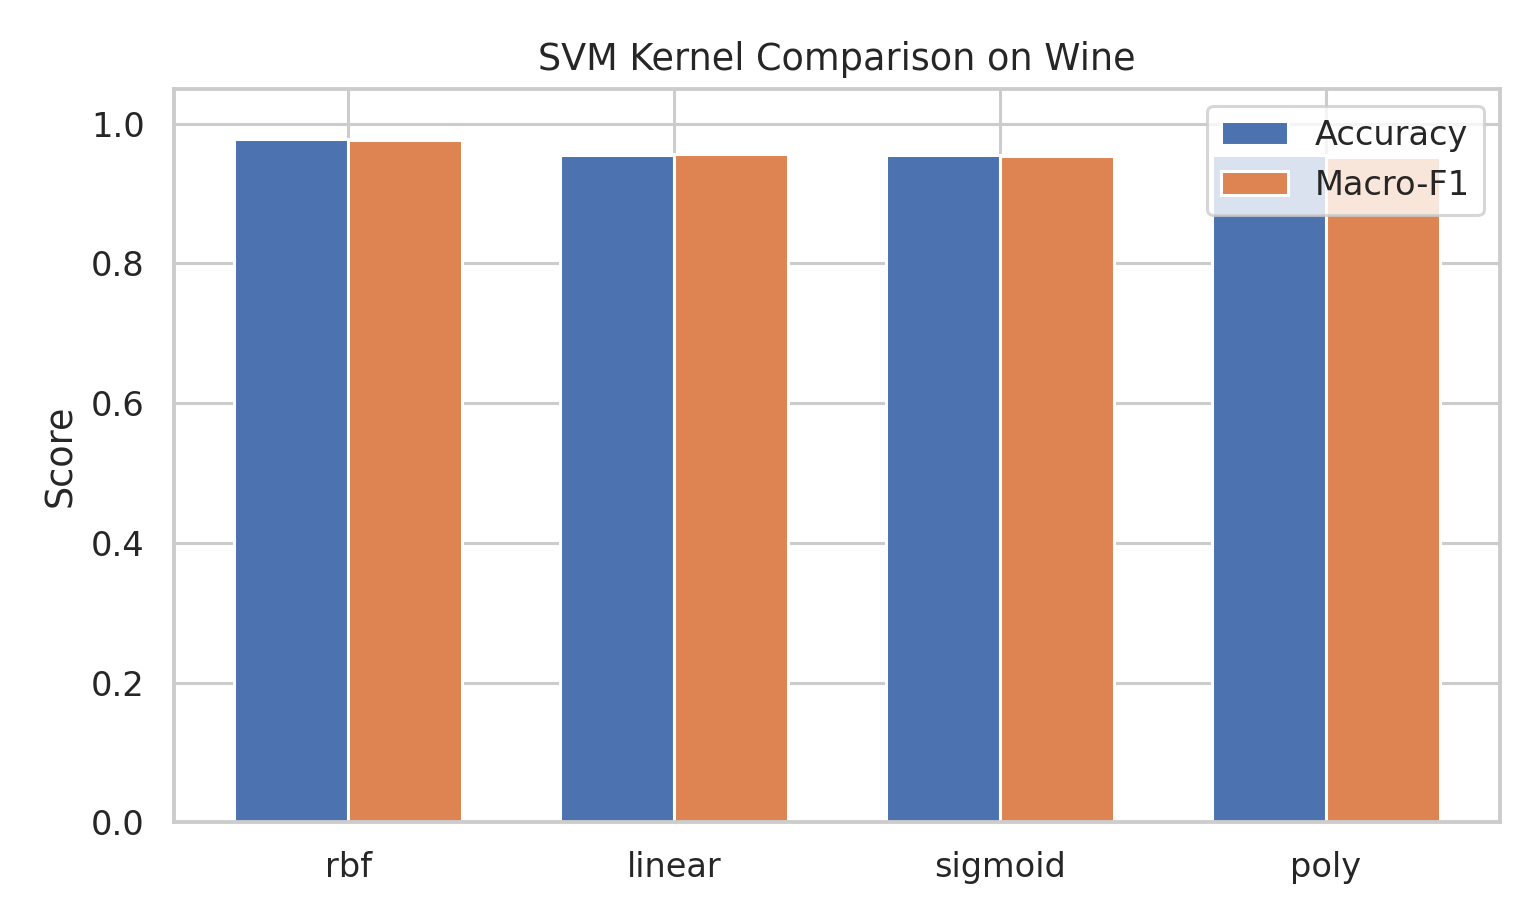
\includegraphics[width=0.78\linewidth]{../results/figures/svm_wine_kernel_comparison.png}
\caption{Wine 数据集上 SVM 核函数比较}
\label{fig:svm-kernel}
\end{figure}

该结果表明，Wine 数据集中的类别边界并非严格线性可分。RBF 核通过局部径向响应构造更灵活的决策边界，因此在较低运行开销下取得了最高的分类性能。

\subsection{RBF 网络的中心数敏感性}
RBF 网络的关键超参数是隐层中心数。若中心过少，模型表达能力不足；若中心过多，模型容易冗余甚至受到样本划分偶然性的影响。表 \ref{tab:rbf-center} 和图 \ref{fig:rbf-center} 展示了中心数扫描结果。

\begin{table}[H]
\centering
\caption{Wine 数据集上 RBF 网络的隐层中心数比较}
\label{tab:rbf-center}
\small
\begin{tabular}{cccc}
\toprule
中心数 & Accuracy & Macro-F1 & 运行时间/s \\
\midrule
6 & 0.9778 & 0.9765 & 0.0209 \\
9 & 1.0000 & 1.0000 & 0.0281 \\
12 & 0.9556 & 0.9522 & 0.0329 \\
15 & 0.9556 & 0.9522 & 0.0382 \\
18 & 0.9778 & 0.9765 & 0.0433 \\
24 & 0.9556 & 0.9522 & 0.0553 \\
30 & 0.9778 & 0.9765 & 0.0662 \\
\bottomrule
\end{tabular}
\end{table}

\begin{figure}[H]
\centering
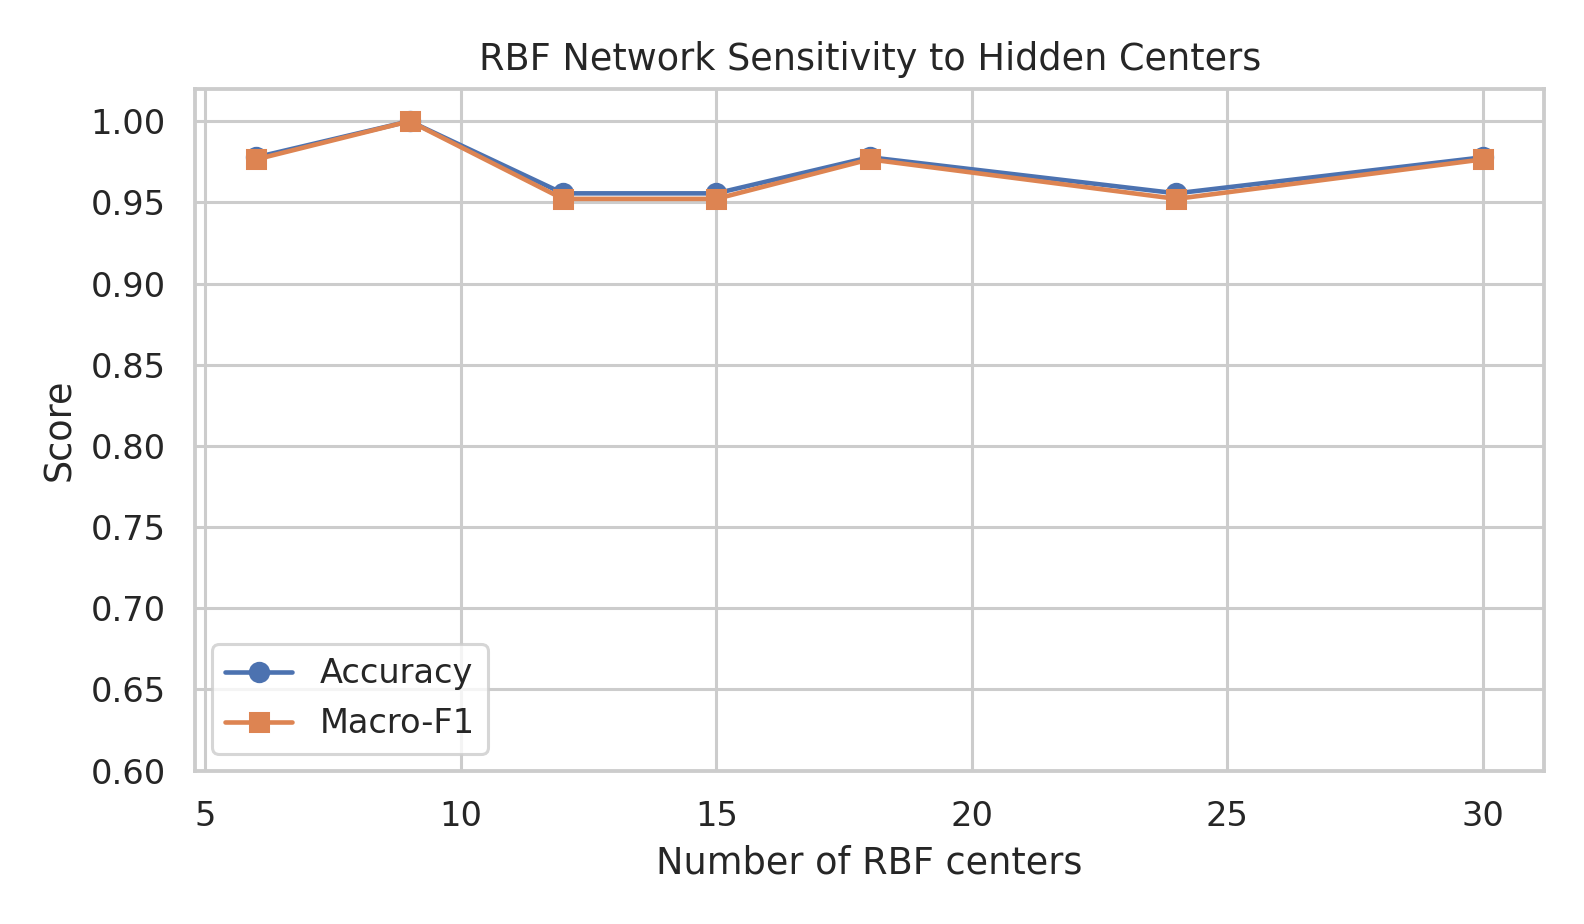
\includegraphics[width=0.78\linewidth]{../results/figures/rbf_wine_center_sweep.png}
\caption{Wine 数据集上 RBF 网络对中心数的敏感性}
\label{fig:rbf-center}
\end{figure}

结果表明，中心数并非单调增大越优。9 个中心对应最高测试性能，而 12、15 和 24 个中心对应的性能反而下降。对于小规模表格数据，RBF 网络的表达能力与泛化能力之间存在明显平衡点。课程课件中关于“中心选取对 RBF 性能具有重要影响”的结论在本实验中得到了验证。

\subsection{BP 网络的结构比较}
BP 网络部分额外比较了 3 种多层感知机结构，结果见表 \ref{tab:mlp-arch} 和图 \ref{fig:mlp-arch}。总体上，更深的网络带来更高的准确率，但也显著增加训练时间。

\begin{table}[H]
\centering
\caption{Fashion-MNIST 子集上不同 BP/MLP 结构比较}
\label{tab:mlp-arch}
\small
\begin{tabular}{lcccc}
\toprule
网络结构 & Accuracy & Macro-F1 & Epochs & 运行时间/s \\
\midrule
MLP(128) & 0.8528 & 0.8521 & 22 & 1.6840 \\
MLP(256,128) & 0.8610 & 0.8606 & 18 & 2.7123 \\
MLP(256,128,64) & 0.8628 & 0.8631 & 30 & 4.9841 \\
\bottomrule
\end{tabular}
\end{table}

\begin{figure}[H]
\centering
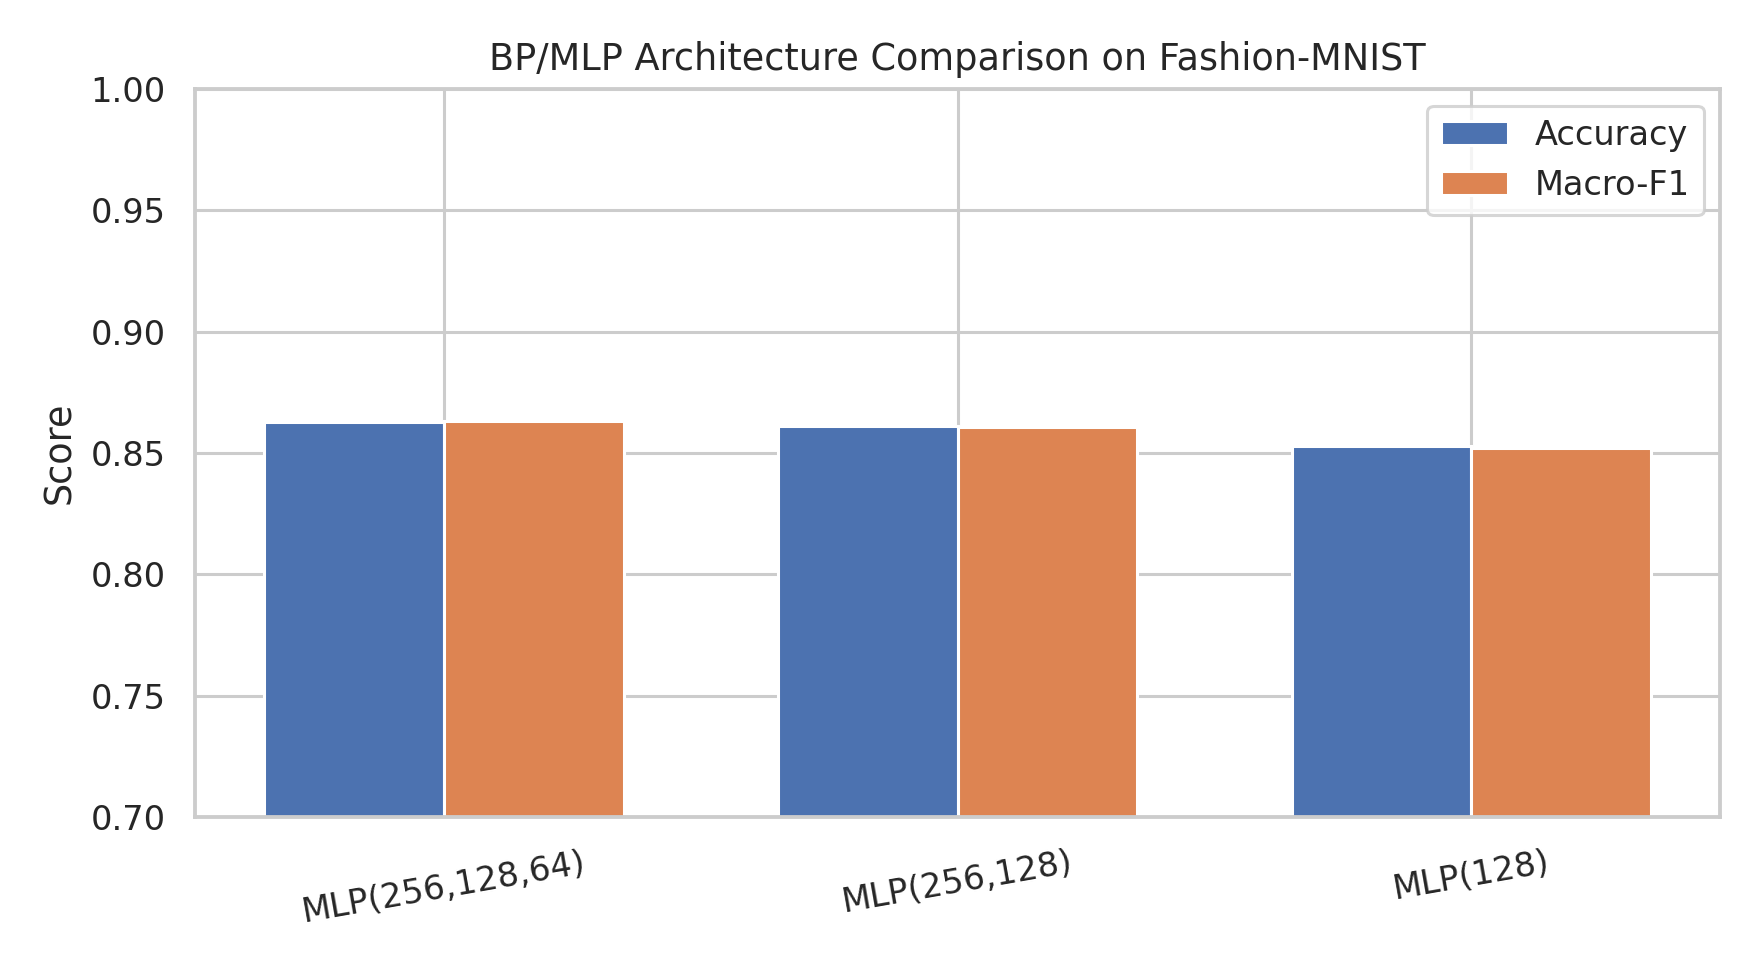
\includegraphics[width=0.82\linewidth]{../results/figures/mlp_fashion_architecture_comparison.png}
\caption{Fashion-MNIST 子集上的 BP/MLP 结构比较}
\label{fig:mlp-arch}
\end{figure}

与单层隐藏结构相比，增加网络深度后，模型对高维图像特征的表达能力增强，准确率有所提升。但从运行时间看，性能最高结构的训练时间约为最浅结构的 3 倍。若同时考虑精度与计算成本，\texttt{MLP(256,128)} 在两者之间表现出较平衡的结果；若优先考虑测试性能，则 \texttt{MLP(256,128,64)} 更合适。

\section{综合讨论}

\subsection{不同算法的适用场景}
综合全部实验，可以得到以下认识。
\begin{itemize}
\item K-means 可用于分析数据中的天然结构，但其优化目标并不直接对应真实标签，因此聚类质量不能简单等同于分类精度。
\item SVM 适用于处理中小规模表格数据，在核函数选取得当时能够以较低时间开销获得较高性能。
\item RBF 网络以“先局部表示、后线性判别”的方式完成分类，在该 Wine 数据划分下其测试性能高于 SVM。
\item BP 网络具有较强的通用逼近能力，能够处理高维图像输入，但需要更多训练样本和更长训练时间。
\end{itemize}

\subsection{实验结论的边界}
尽管实验结果具有一定区分度，但仍需注意其适用边界。首先，Wine 数据集样本量较小，单次训练/测试划分下出现 100\% 准确率并不意味着模型在更一般情形下一定优于其他方法，后续可通过增加交叉验证提高结论稳健性。其次，Fashion-MNIST 上使用的仍然是全连接 BP 网络，而非卷积网络，因此性能存在上限。再次，K-means 的结果受初始化、簇数和特征变换影响较大，若采用更多随机种子重复试验，结论将更加稳健。

\subsection{与课程内容的对应关系}
本报告的实验设计与课程内容具有明确对应关系。K-means 对应“非监督分类与聚类”课件，SVM 对应“线性分类与支持向量机”课件，BP 网络和 RBF 网络分别对应“常用人工神经网络”课件中的两类核心模型。同时，RBF 网络中用 K-means 选中心的实现方式，也体现了课程不同章节之间的内在联系。整体上，本文形成了“课件方法 - 代码实现 - 实验比较 - 结果分析”的完整实验流程。

\section{结论}
本文以课程课件中的典型算法为基础，完成了 K-means、SVM、BP 网络和 RBF 网络四类方法的统一仿真，并在主实验之外加入了 4 组附加对比实验。实验结果表明：
\begin{itemize}
\item K-means 在 Iris 数据集上能够反映样本的天然结构，但聚类评估需要同时关注内部指标与外部指标。
\item RBF 核 SVM 是 Wine 数据上的强基线模型，准确率达到 97.78\%。
\item 基于 K-means 选中心的 RBF 网络在 Wine 数据集上表现极优，9 个中心时达到 100\% 准确率。
\item BP 网络在 Fashion-MNIST 子集上具备良好的图像分类能力，增加网络深度可以换取一定精度提升，但代价是更长训练时间。
\end{itemize}

后续工作可以从两个方向继续推进。第一，将课程中的 Fisher 判别、PCA、EM、SOM 等算法纳入同一实验框架，形成更完整的课程算法库。第二，在图像分类部分进一步引入卷积神经网络，对比 BP 网络与 CNN 在 Fashion-MNIST 或更复杂数据集上的差异。

\appendix
\section{复现实验所用文件说明}
附录列出主要文件位置。
\begin{itemize}
\item 主脚本：\texttt{scripts/run\_all.py}
\item RBF 网络实现：\texttt{src/ml\_course/rbf\_network.py}
\item 实验逻辑：\texttt{src/ml\_course/experiments.py}
\item 结果图表：\texttt{results/figures/} 与 \texttt{results/tables/}
\end{itemize}

\begin{thebibliography}{99}

\bibitem{macqueen1967}
J. MacQueen.
\newblock Some Methods for Classification and Analysis of Multivariate Observations.
\newblock In \emph{Proceedings of the Fifth Berkeley Symposium on Mathematical Statistics and Probability}, Volume 1, pages 281--297, 1967.

\bibitem{cortes1995svm}
Corinna Cortes and Vladimir Vapnik.
\newblock Support-Vector Networks.
\newblock \emph{Machine Learning}, 20(3):273--297, 1995.

\bibitem{rumelhart1986bp}
David E. Rumelhart, Geoffrey E. Hinton, and Ronald J. Williams.
\newblock Learning Representations by Back-Propagating Errors.
\newblock \emph{Nature}, 323:533--536, 1986.

\bibitem{moody1989rbf}
John Moody and Christian J. Darken.
\newblock Fast Learning in Networks of Locally-Tuned Processing Units.
\newblock \emph{Neural Computation}, 1(2):281--294, 1989.

\bibitem{fisher1936iris}
R. A. Fisher.
\newblock The Use of Multiple Measurements in Taxonomic Problems.
\newblock \emph{Annals of Eugenics}, 7(2):179--188, 1936.

\bibitem{uciiris}
UCI Machine Learning Repository.
\newblock Iris Dataset.
\newblock DOI: \url{https://doi.org/10.24432/C56C76}.

\bibitem{uciwine}
UCI Machine Learning Repository.
\newblock Wine Dataset.
\newblock DOI: \url{https://doi.org/10.24432/C5PC7J}.

\bibitem{xiao2017fashion}
Han Xiao, Kashif Rasul, and Roland Vollgraf.
\newblock Fashion-MNIST: a Novel Image Dataset for Benchmarking Machine Learning Algorithms.
\newblock \emph{arXiv preprint arXiv:1708.07747}, 2017.

\end{thebibliography}

\end{document}
